\section{Desenvolvimento}
Neste capítulo, serão apresentados os principais detalhes sobre o desenvolvimento do protótipo. Todos os códigos, diagramas esquemáticos e todos os detalhes para preparação da infraestrutura de software, estão disponíveis em um repositório no GitHub\footnote{URL: https://github.com/danielgoncalves/iot-ifsp-ctd-tcc. Acesso em: 25 nov. 2024.} dedicado a este trabalho de conclusão de curso.

\subsection{Unidades}
O sistema em questão consiste em três conjuntos principais, ou unidades distintas: 
\begin{itemize}
    \item Unidade de Monitoramento e Comando
    \item Unidade de Medição
    \item Unidade de Escoamento ou Alimentação
\end{itemize}

\subsection{Unidade de Monitoramento}
A Unidade de Monitoramento é composta por um módulo ESP32, um mostrador de cristal líquido de 16x2 (16 colunas por 2 linhas) e 3 botões de pressionamento. Como o nome sugere, sua função é receber os dados dos tópicos MQTT onde são publicados valores de leitura dos níveis pelas Unidades de Medição, além de possibilitar o ajuste do nível crítico de cada Unidade de Medição e de, opcionalmente, comandar manualmente o escoamento de uma determinada Unidade de Escoamento. Figuras \ref{fig:photo-monitoring-unit} e \ref{fig:schematic-monitoring-unit}.

\begin{figure}[h!]
    \centering
    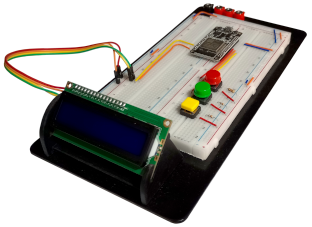
\includegraphics[width=7cm]{imagem/unidade-monitoramento.png}
    \caption{Protótipo da Unidade de Monitoramento}
    \label{fig:photo-monitoring-unit}
\end{figure}

\begin{figure}[h!]
    \centering
    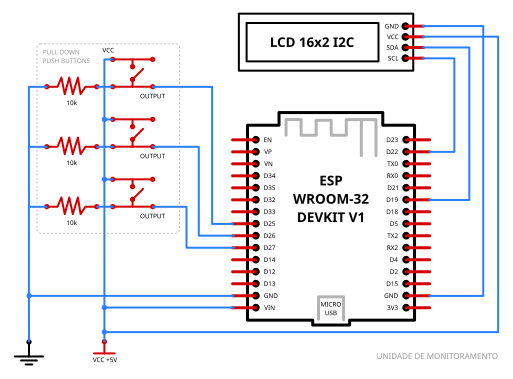
\includegraphics[width=9cm]{imagem/diagrama-unidade-monitoramento.png}
    \caption{Esquemático da Unidade de Monitoramento}
    \label{fig:schematic-monitoring-unit}
\end{figure}

\subsection{Unidade de Medição}
A Unidade de Medição é composta por um módulo ESP32 e um sensor ultrassônico HC-SR04. Pela proposta do trabalho, pode-se ter apenas uma Unidade de Medição ou várias. Para este trabalho foram desenvolvidas duas unidades para medição de dois conjuntos de contêineres. Sua função é medir o nível de um tanque ou contêiner e, atingido um determinado nível, que é configurado na própria unidade (ou através da Unidade de Monitoramento), é comandado escoamento de forma remota via MQTT. Figuras \ref{fig:photo-measure-unit} e \ref{fig:schematic-measure-unit}.

\begin{figure}[h!]
    \centering
    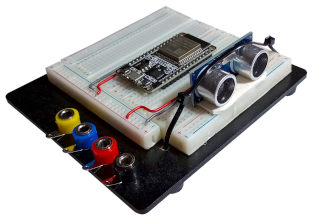
\includegraphics[width=7cm]{imagem/unidade-medicao.png}
    \caption{Protótipo da Unidade de Medição}
    \label{fig:photo-measure-unit}
\end{figure}

\begin{figure}[h!]
    \centering
    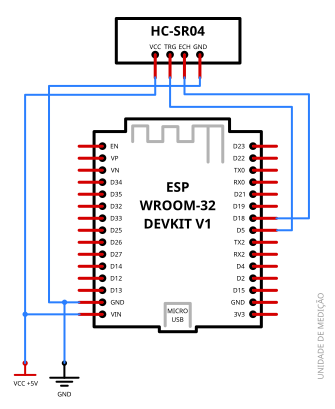
\includegraphics[width=7cm]{imagem/diagrama-unidade-medicao.png}
    \caption{Esquemático da Unidade de Medição}
    \label{fig:schematic-measure-unit}
\end{figure}

\subsection{Unidade de Escoamento}
A Unidade de Escoamento é composta por um módulo ESP32, um transistor TP41C NPN, e uma mini bomba d'água. O acionamento da bomba d'água é feito quando a unidade recebe uma mensagem MQTT indicando o tempo, em segundos, que a bomba deverá permanecer acionada. Figuras \ref{fig:photo-pump-unit} e \ref{fig:schematic-pump-unit}.

\begin{figure}[h!]
    \centering
    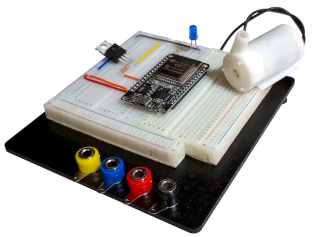
\includegraphics[width=7cm]{imagem/unidade-escoamento.png}
    \caption{Protótipo da Unidade de Escoamento}
    \label{fig:photo-pump-unit}
\end{figure}

\begin{figure}[h!]
    \centering
    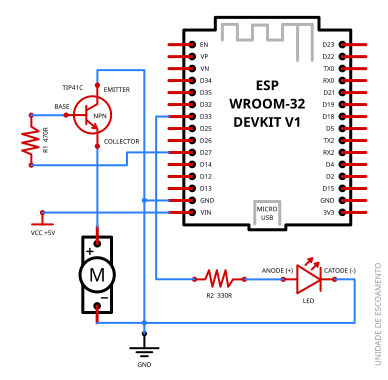
\includegraphics[width=0.5\linewidth]{diagrama-unidade-escoamento.png}
    \caption{Esquemático da Unidade de Escoamento}
    \label{fig:schematic-pump-unit}
\end{figure}

\subsection{Protótipo Montado}
A figura \ref{fig:mounted-aparatus} mostra as unidades protótipo, montadas próximas para facilitar o entendimento do aparato de hardware. Neste caso, a imagem mostra apenas uma unidade de medição e uma unidade de escoamento. Quando o contêiner que está sob a unidade de medição atinge o nível configurado, é comandado o escoamento para o contêiner ao lado.

\begin{figure}[h!]
    \centering
    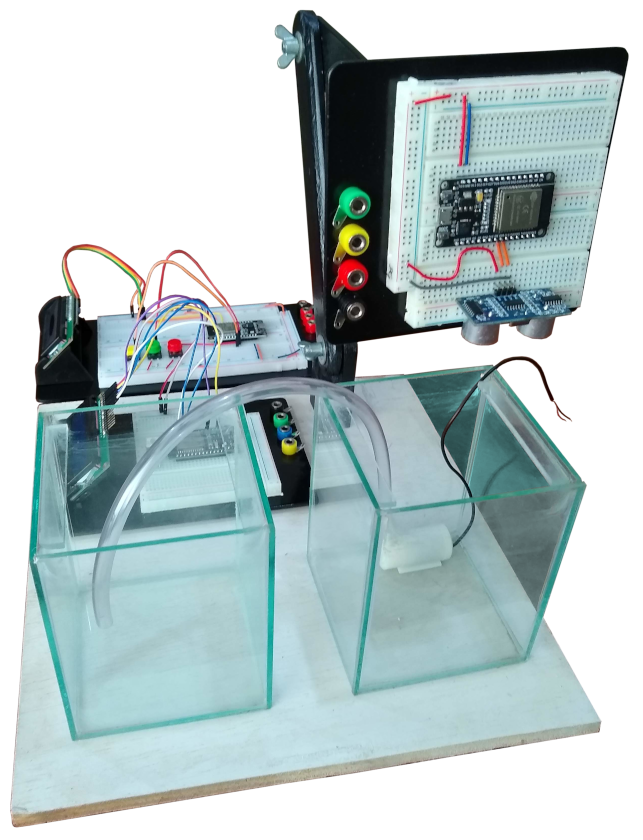
\includegraphics[width=11cm]{imagem/prototipo-montado-1.png}
    \caption{Unidades posicionadas próximas}
    \label{fig:mounted-aparatus}
\end{figure}

\subsection{Software}
Os códigos-fonte das unidades foram escritos em C++ (na verdade, abstrações em C++ sobre a linguagem Wiring\footnote{URL: https://wiring.org.co/. Acesso em: 31 ago. 2023.}) através do ambiente integrado de desenvolvimento (IDE) para Arduino\footnote{URL: https://www.arduino.cc/en/software}. 

\subsection{Infraestrutura para Comunicação}
A comunicação entre as unidades ocorre através do protocolo MQTT. Para isso é necessário um software servidor que implemente o protocolo MQTT. Neste projeto utilizamos a implementação do Eclipse Mosquitto. 

\subsection{Infraestrutura para Logging e Monitoramento}
As leituras feitas pelas unidades de medição ficam registradas em um banco de dados relacional (RBDMS) PostgreSQL. O registro das leituras é feito por um fluxo específico, através da plataforma Node-RED, onde os dados que chegam no tópico "p/container/level"\space são registrados em uma tabela específica.
Também através da plataforma Node-RED, foram implementados fluxos para visualização dos níveis dos contêineres em um painel de instrumentação (\textit{dashboard}) que pode ser visualizado através de um navegador de internet (\textit{web browser}, figura \ref{fig:dashboard-node-red}). O fluxo Node-RED utilizado está disponível no repositório do projeto em \url{https://github.com/danielgoncalves/iot-ifsp-ctd-tcc/blob/main/Infra/Node-RED/flow.json}, figura \ref{fig:node-red-ui}.

\begin{figure}[h!]
    \centering
    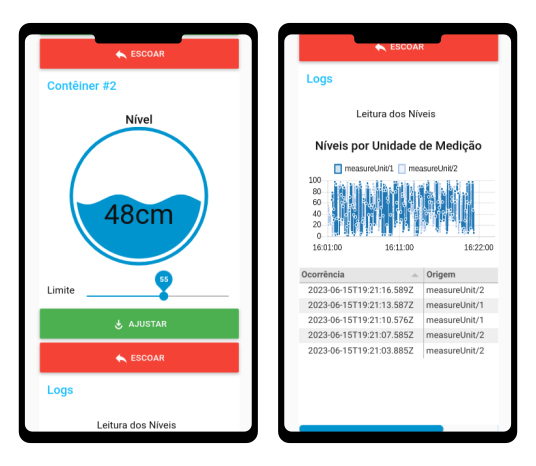
\includegraphics[width=12cm]{imagem/dashboard-mobile.png}
    \caption{Dashboard implementado via Node-RED}
    \label{fig:dashboard-node-red}
\end{figure}

\begin{figure}[h!]
    \centering
    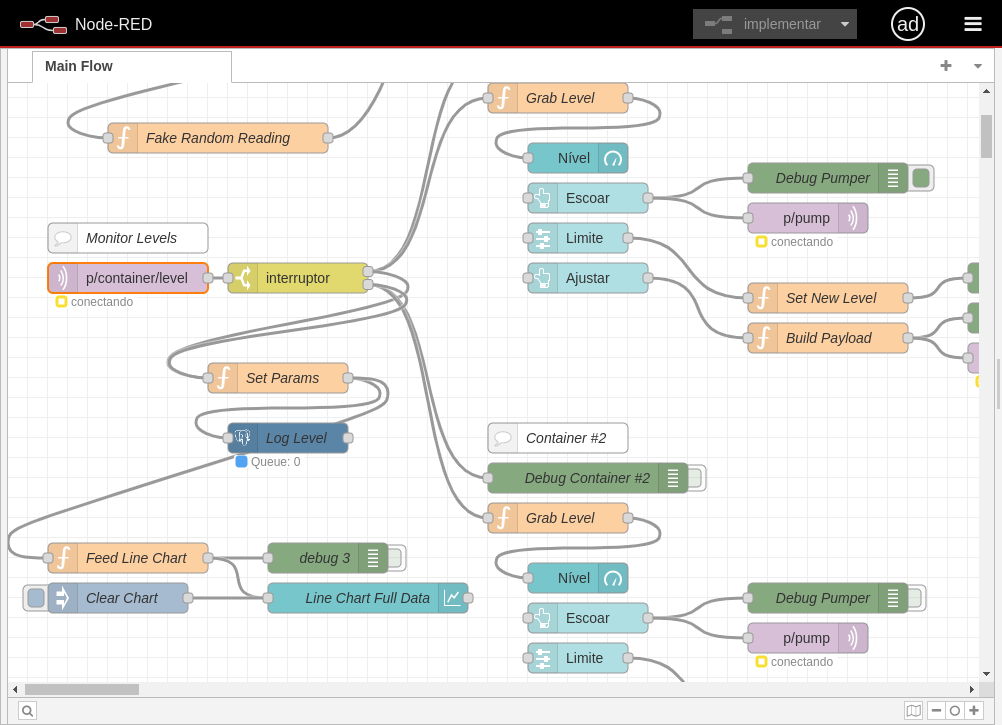
\includegraphics[width=0.5\linewidth]{imagem/node-red-ui.png}
    \caption{Interface do Node-RED com o fluxo deste projeto}
    \label{fig:node-red-ui}
\end{figure}

\subsection{Implementação da Infraestrutura}
Para disponibilizar os serviços de software citados nos tópicos anteriores, optou-se por utilizar virtualização baseada em \textit{containers} Docker\footnote{URL: https://docs.docker.com/}. Por serem relativamente leves, é possível executar todos os serviços necessários em um único hospedeiro baseado em Linux, e testar toda a implementação do projeto em rede local.

Porém, essa mesma infraestrutura pode ser disponibilizada em uma instância AWS EC2\footnote{URL: https://aws.amazon.com/pt/ec2/} e ter os serviços disponibilizados de forma ampla via internet.

\clearpage

